\section{Simulated AT-TPC events}
The simulated AT-TPC tracks were simulated with the \lstinline{pytpc} package developed at the NSCL\todo{citation}. Using the same parameters as for the $Ar^{46}(p, p)$ experiment a set of $N=4000$ events were generated per class. The events are generated in the same format as the semi-raw experimental data. That is they are represented as peak-only 4-tuples of $e_i = (x_i, y_i, t_i, c_i)$. Each event is then a set of these four-tuples: $\epsilon_j = \{e_i\}$ creating a track in three dimensional space with charge amplitude for each point. To process these events with the algorithms implemented for this thesis we chose to represent these 3D tracks as 2D images with charge represented as pixel images. For the analysis we chose to view the x-y projection of the data \todo{figure of 3D simulated track and 2D representation}

\subsection{Classification of events} 
From the simulated data we have two classes of events; proton and carbon. Our hypothesis is that we can separate these with a linear classifier, additionally we will investigate how many labeled samples we need to achieve good classification. The investigation of the performance will be separated in the sequential and non\-sequential models. The simulated data is very simple and does not necessitate the full hyperparameter search machinery. We begin by considering the non-sequential Autoencoders.

\subsubsection{Convolutional Autoencoder classification results\protect\footnote{The scripts used to produce the results for this section can be found in the repository at: \lstinline{scripts/convae_simulated.py}, \lstinline{notebooks/draw_model.ipynb}, and \lstinline{notebooks/latent_space_simulated.ipynb}}}

The training procedure for classification using a semi-supervised regime as the one we'll apply necessitates the same strict separation of labeled data for the classification step as when considering ordinary classification tasks. To emulate the real-data case we set a subset of the simulated data to be labeled and treat the rest as unlabeled data. We chose this partition to be $15\%$ of each class. We denote this subset and its associated labels as $\gamma_L=(\mathbf{X}_L, \mathbf{y}_L)$, the entire dataset which we will denote as $\mathbf{X}_F$. To clarify please note that $\mathbf{X}_L \subset \mathbf{X}_F$. Furthermore, the tuple $\gamma_L$ has to be split in training and test sets. The test partition is set to be $30\%$ of the samples. The hyperparameters were tuned with the \lstinline{RandomSearch} architecture which searches in a semi structured way over all the parameters given in table \ref{tab:convae_hyperparams} we list the experiments with their corresponding proton $f1$ score in appendix \ref{tab:convae_randomsearch}. We optimize the classification performance using $M=40$ semi-structured random experiments. To illustrate the difference in quality and convergence of the runs we show the plot of the resulting loss curves of the highest $N=10$ runs in figure \ref{fig:sim_clf_loss}. In the figure lighter colors represent higher proton $f1$ scores, and as such the same color across the reconstruction and latent losses represent the same experiment. We also denote different scales and corresponding markers for the reconstruction and latent losses. We observe that in the top 10 performing runs there are no versions of the model that maintains a VAE-style Kullback Leibler loss on the latent space. And that the very highest performing model maintains no regularization at all, while considerably more complex than the runners up as seen from appendix \ref{tab:convae_randomsearch}.

\begin{figure}[H]
\centering
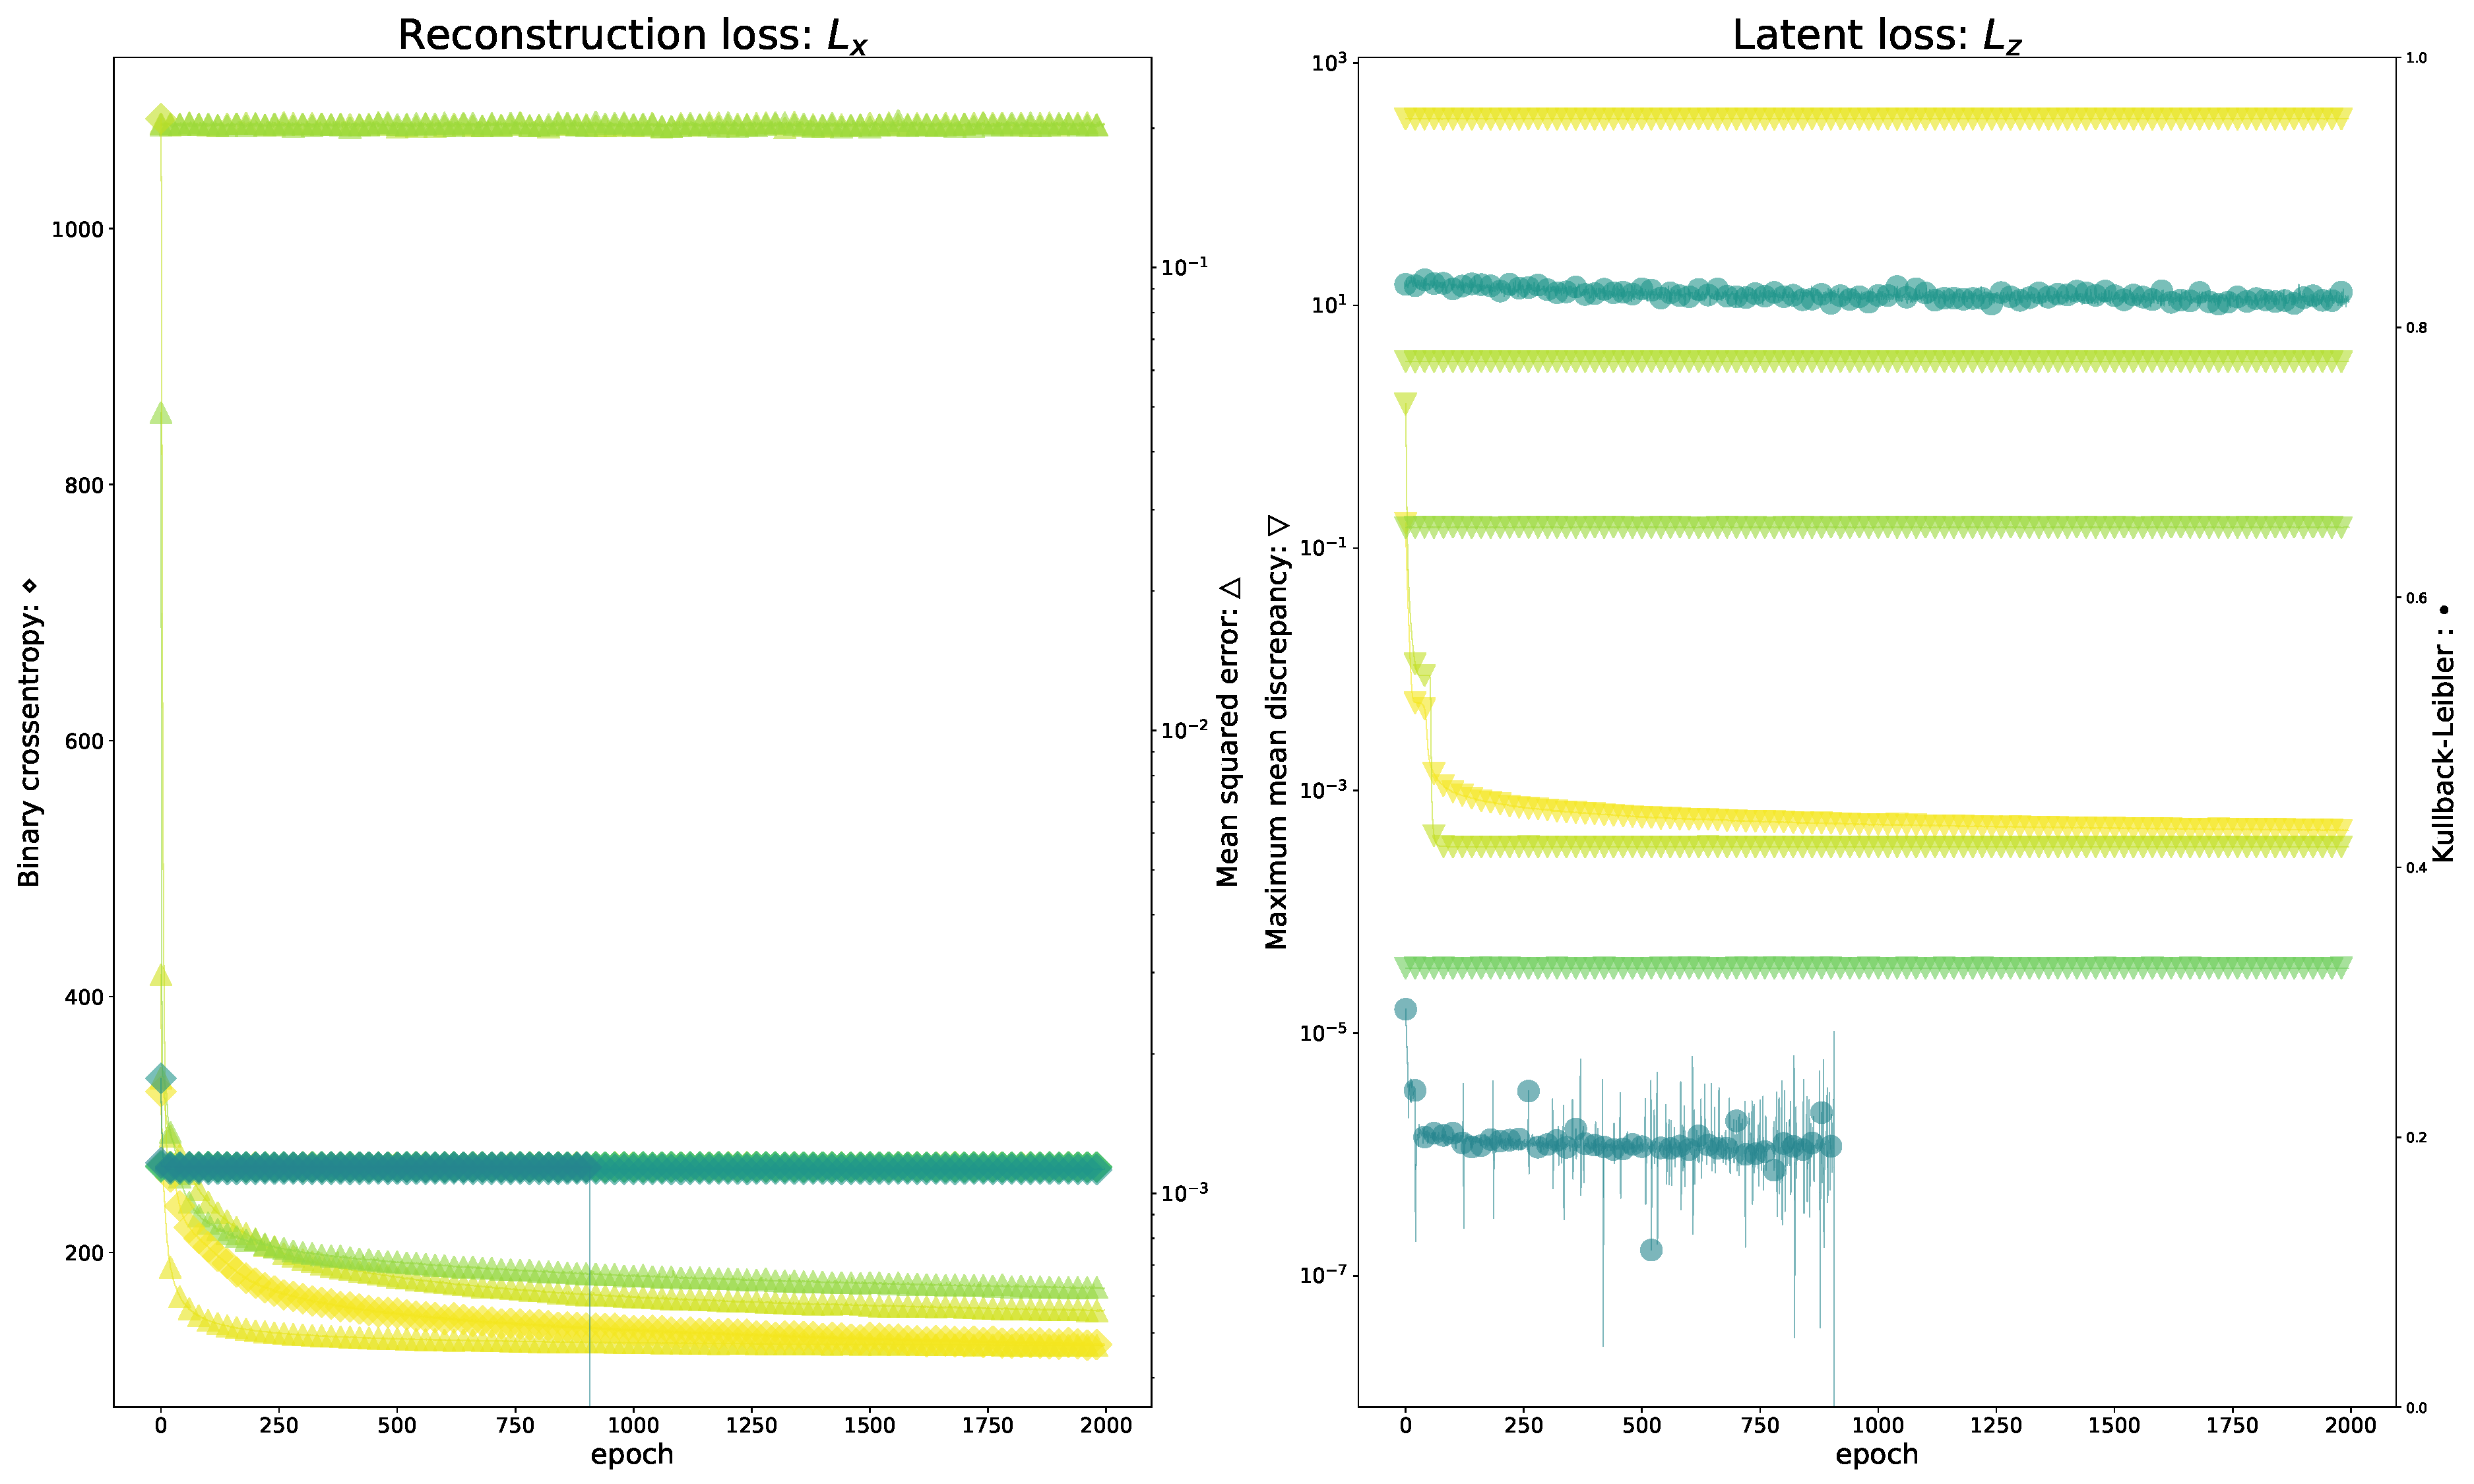
\includegraphics[width=\textwidth]{/plots/randomsearch_loss.pdf}
\caption[Randomsearch loss curves for CONV-AE on simulated AT-TPC data]{Distribution of the $N=10$ best loss curves from $M=40$ experiments with a convolutional autoencoder. Lighter colors indicate higher proton $f1$ scores, and as such there is an implied 1-1 correspondence between the plots. The lightest colored line represents a proton score of $f1_p = 0.98$, implying near perfect classification. While the worst performing model included in the plot has a score of $f1_p = 0.92$. The line-markers denote the loss-type for the associated run, with the axis the run is plotted on containing the corresponding legend. We observe that the maximum-mean-discrepancy loss on the latent distribution consistently outperforms the Kullback Leibler loss as none are included in the top 10. The full table is listed in appendix \ref{tab:convae_randomsearch}}\label{fig:sim_clf_loss}
\end{figure}


The classifier was a logistic regression model from the \lstinline{scikit-learn} python library trained on the latent expressions of the train partition of $\mathbf{X}_L$. The hyperparameters of the best performing model, with the least complexity, is listed in table \ref{tab:param_vals_sim_convae}. We chose a simpler model as it has fewer variables to fit and as such it is less prone to overfitting effects unsupervised models can exhibit. 


\begin{table}
\centering
\setlength{\extrarowheight}{15pt}
\hspace*{-0.5in}
\begin{tabular}{ll}
\toprule
Hyperparameter & Value \\
\midrule
\multicolumn{2}{l}{Convolutional parameters: } \\
\midrule
Number of layers & 3\\
Kernels & $[11,\, 5,\, 3]$\\
Strides & $[2,\, 2,\, 2]$\\
Filters & $[16,\, 16,\, 8]$ \\ 
\midrule
\multicolumn{2}{l}{Network parameters: } \\
\midrule
Activation & ReLU \\
Latent type & MMD \\
Latent dimension & $3$ \\
$\beta$ & \num{10} \\
\midrule
\multicolumn{2}{l}{Optimizer parameters: } \\
\midrule
$\eta$ &  \num{1e-1} \\
$\beta_1$ & $0.55$ \\
$\beta_2$ & $0.99$ \\
\bottomrule
\end{tabular}
\caption{Hyperparameters that gives the strongest performance with the least complexity on the simulated events. The configuration chosen is listed in appendix \ref{tab:convae_randomsearch}}\label{tab:param_vals_sim_convae}
\end{table}

Furthermore we wish to estimate the variability of the highest performing model. To achieve this we then re-ran the convolutional autoencoder $N=10$ times using the configuration listed in table \ref{tab:param_vals_sim_convae}. The model performs strongly with very little variation in the proton $f1$ scores. We list the $f1$ scores by class in table \ref{tab:clf_simulated} and display the associated loss curves in figure \ref{fig:best_model_sim_clf}.

\begin{figure}[H]
\centering
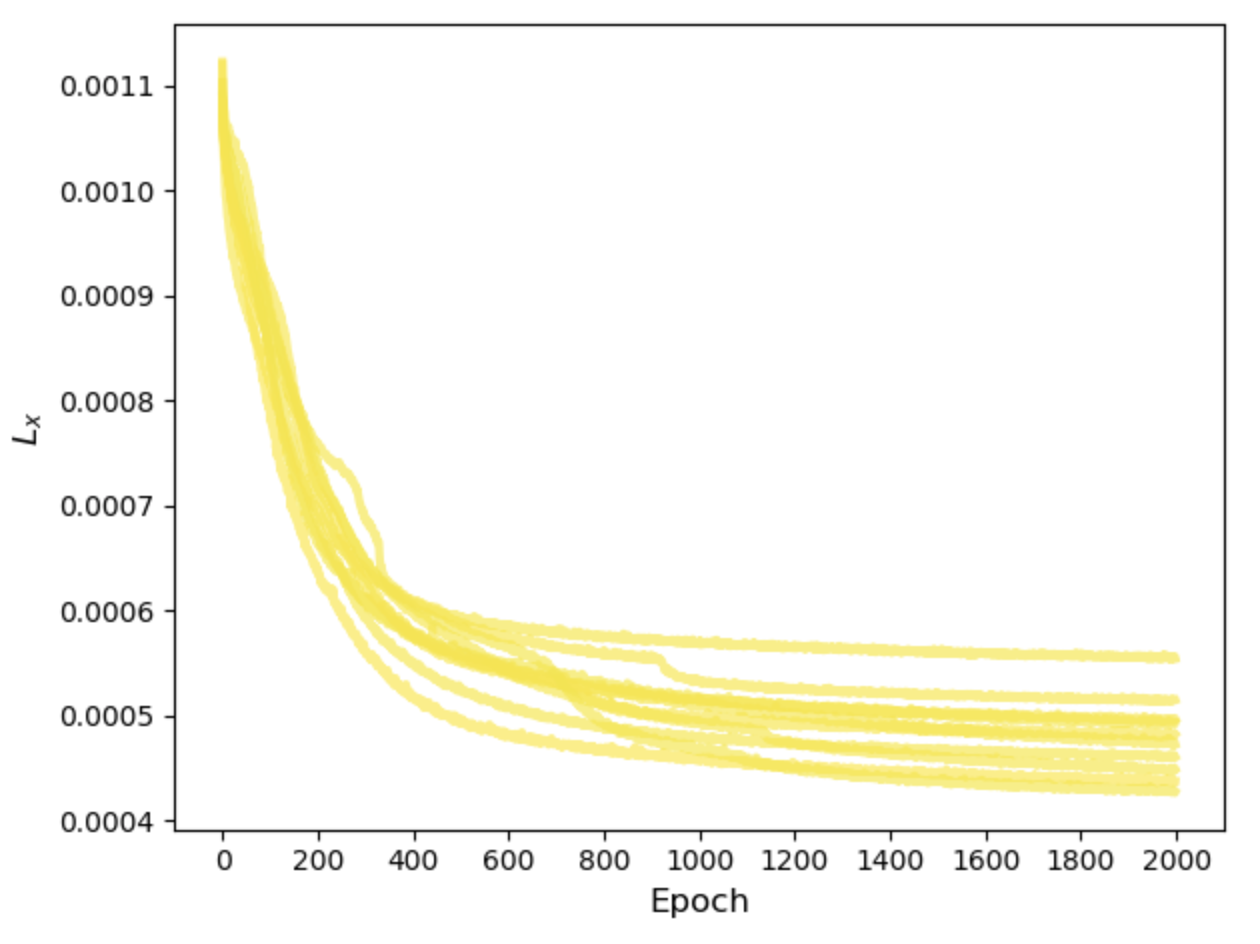
\includegraphics[width=\textwidth, height=4in]{plots/reconst_best_model_simulated.png}
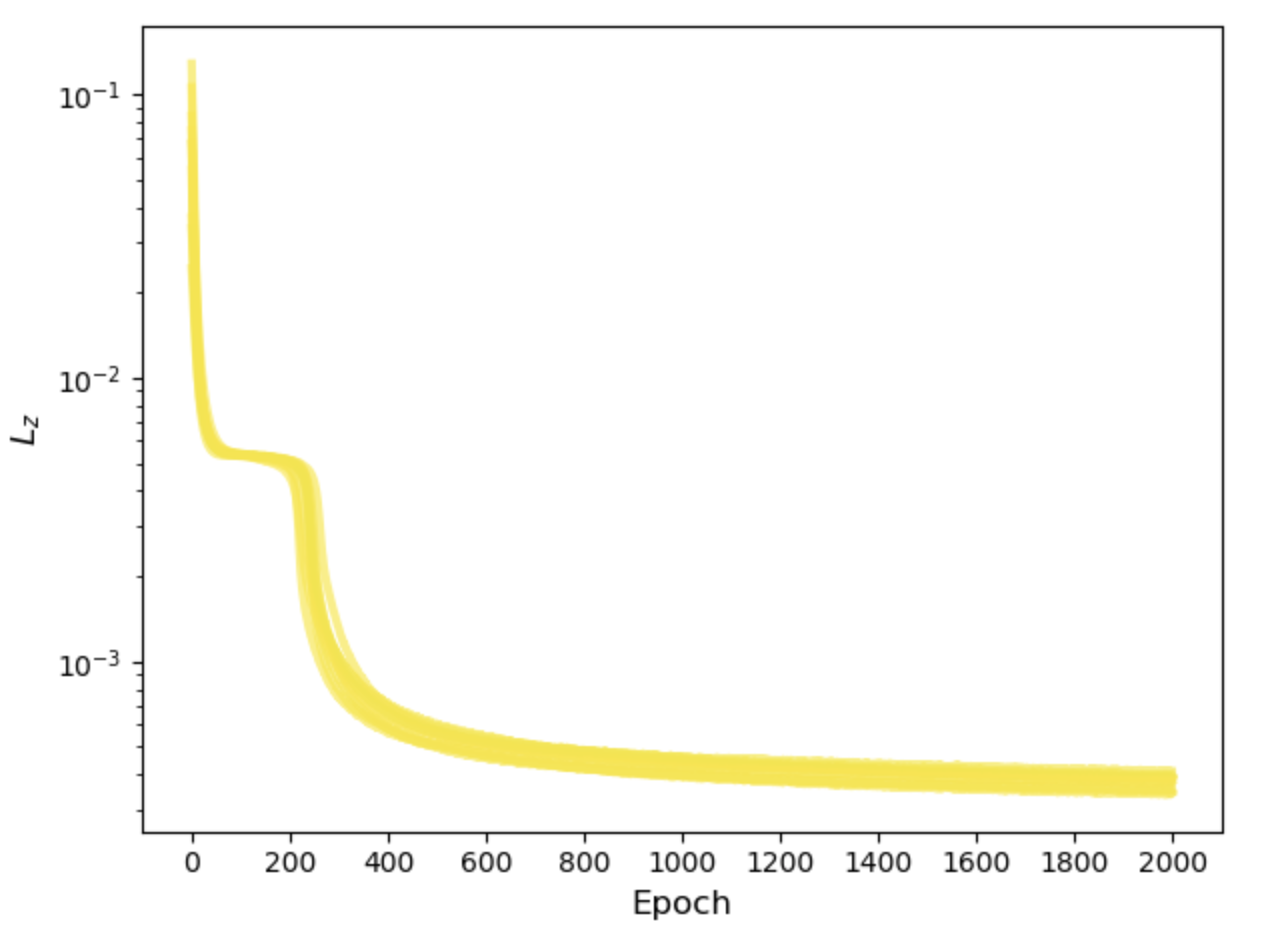
\includegraphics[width=\textwidth, height=4in]{plots/latent_best_model_simulated.png}
\caption[$L_x$ and $L_z$ for the CONV-AE on simulated AT-TPC data]{Reconstruction and latent loss curves for the $N=10$ runs of the best performing convolutional autoencoder using the configuration listed in table \ref{tab:param_vals_sim_convae}. The lightness of color indicates the proton $f1$ score achieved by the given model. The lightest color in the plot corresponds to a score of about $f1_p = 0.98$.}\label{fig:best_model_sim_clf}
\end{figure}

\begin{table}
\begin{tabular}{lcccccc}
\toprule
{} & \multicolumn{3}{c}{Proton} & \multicolumn{3}{c}{Carbon} \\  
\midrule
 & f1 & recall & precision & f1 & recall & precision\\  
 Train & $ \underset{ \num{+- 7.03e-02 } } {\num{ 0.88 } }  $ & $ \underset{ \num{+- 5.93e-02 } } {\num{ 0.88 } }  $ & $ \underset{ \num{+- 8.56e-02 } } {\num{ 0.86 } }  $ & $ \underset{ \num{+- 4.39e-02 } } {\num{ 0.90 } }  $ & $ \underset{ \num{+- 5.32e-02 } } {\num{ 0.89 } }  $ & $ \underset{ \num{+- 7.37e-02 } } {\num{ 0.87 } }  $ \\ 
  Test & $ \underset{ \num{+- 7.07e-02 } } {\num{ 0.88 } }  $ & $ \underset{ \num{+- 6.40e-02 } } {\num{ 0.89 } }  $ & $ \underset{ \num{+- 7.67e-02 } } {\num{ 0.87 } }  $ & $ \underset{ \num{+- 6.06e-02 } } {\num{ 0.90 } }  $ & $ \underset{ \num{+- 6.80e-02 } } {\num{ 0.89 } }  $ & $ \underset{ \num{+- 7.11e-02 } } {\num{ 0.88 } }  $\\
\bottomrule
\end{tabular}
\caption{Performance as measured by $f1$, precision and recall of the convolutional autoencoder as specified in table \ref{tab:param_vals_sim_convae} on simulated at-tpc data. The standard errors are estimated by running the simulation $N=10$ times with random initialization of weights for each experiment}\label{tab:clf_simulated}
\end{table}

To verify the performance it helps to consider the reconstruction. We would expect a good performing model to be able to reconstruct similar representations to what it was given as input as this structural information then has to have passed through the information bottleneck. In figure \ref{fig:sim_convae_reconstruction} we show that the reconstruction resembles the original strongly, even discerning the minute breaks in the carbon line caused by some aspect of the simulation. While we also note the blurring typical of the pixel-wise reconstruction. 

\begin{figure}
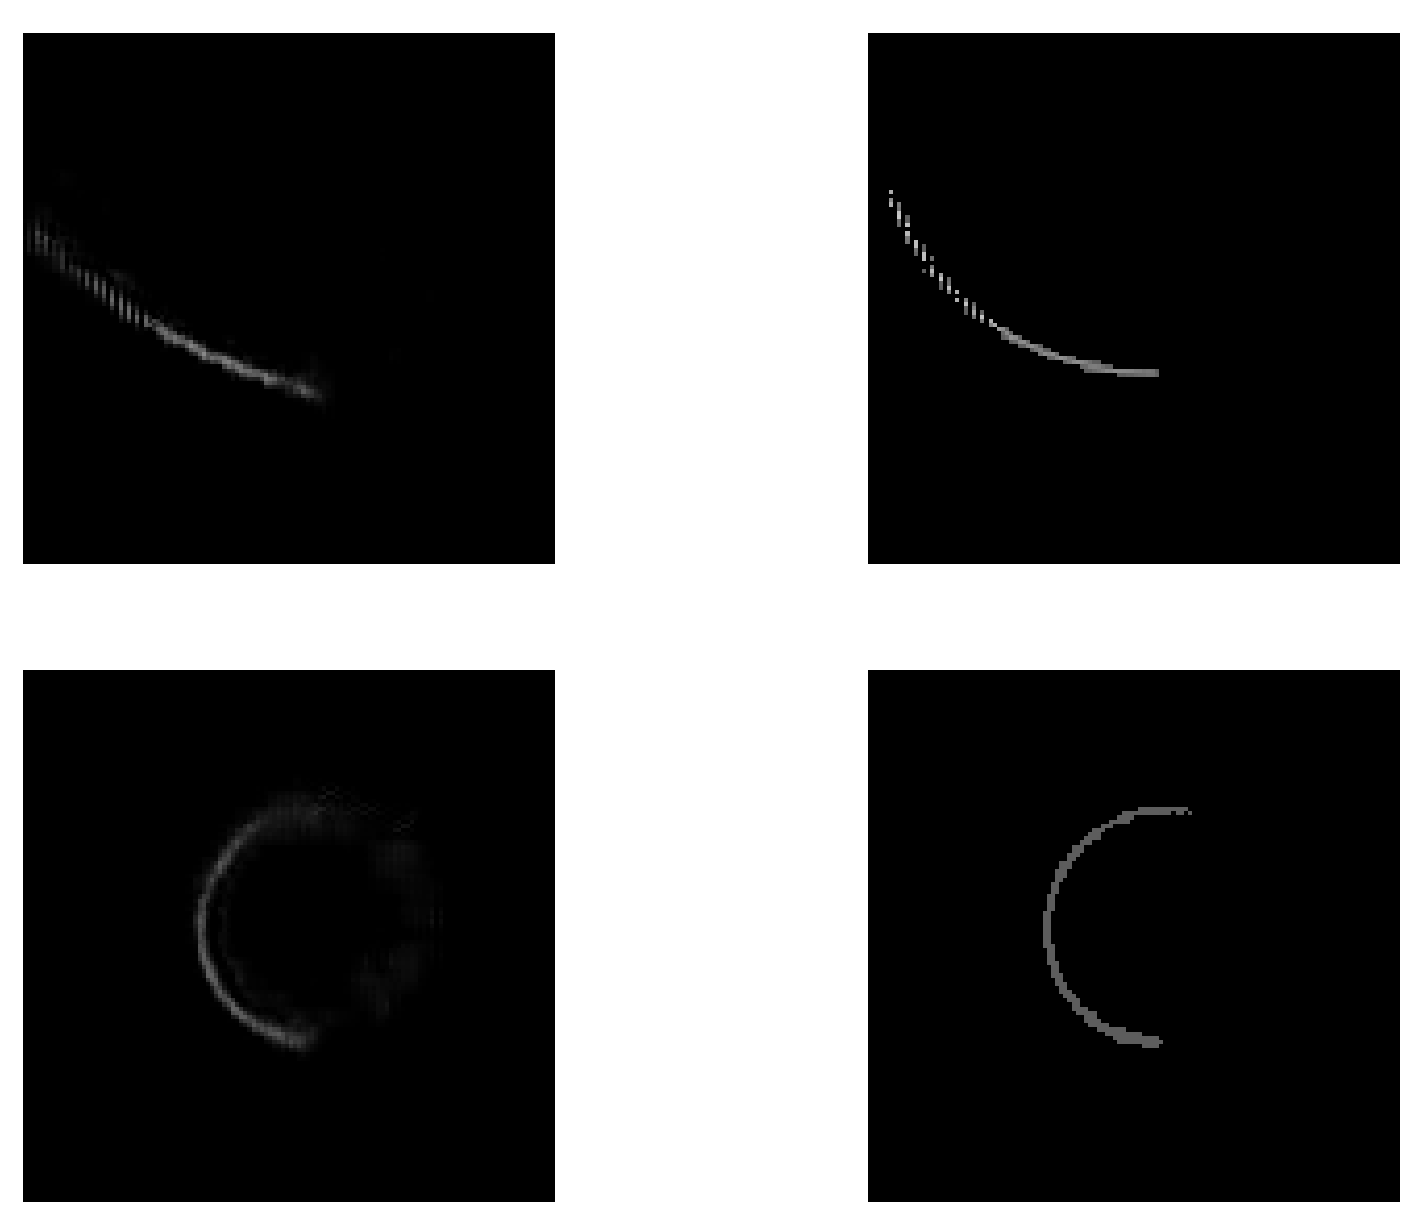
\includegraphics[width=\textwidth, height=4in]{plots/convae_reconstruction.png}
\caption[CONV-AE reconstructions of simulated AT-TPC events]{Reconstructions and inputs produced by the convolutional autoencoder with the configuration listed in table \ref{tab:param_vals_sim_convae}. The left column are the reconstructions of the right column which are model inputs. We note that the model is able to pick up even the breaks in the line-structure from the simulations, and that reconstruction of the proton events exhibit a blurring effect common to pixel wise mse or bce losses.}\label{fig:sim_convae_reconstruction}
\end{figure}

Lastly we investigate the relationship between the hyperparameters and the proton $f1$ score. Among the reasons for using a random-search procedure for the hyperparameter search is the possibly complex, non-monotonic relationships between parameters and the outcome we wish to measure. As such the ordinary tools of estimating correlation and co-variance must come with caveats. Table \ref{tab:hyperparam_corr} of correlation between the parameters and the proton $f1$ score, but we note that while none of the correlations were significant - this may be a consequence of violated assumptions and non-monotonic relationships.

\begin{table}
\centering
\begin{tabular}{lrr}
\toprule
{} &  $\rho_s$ &     p \\
\midrule
proton f1 score  &         1 &     0 \\
N parameters     &      0.36 & 0.079 \\
largest kernel   &      0.38 & 0.058 \\
N layers         &     -0.26 &  0.21 \\
latent dimension &      0.17 &  0.43 \\
batchnorm        &      0.26 &  0.21 \\
$\beta$          &     -0.14 &  0.51 \\
$\beta_1$        &    -0.065 &  0.76 \\
$\eta$           &     -0.14 &  0.51 \\
kld              &     -0.15 &  0.46 \\
mmd              &      0.11 &  0.59 \\
none             &    -0.012 &  0.96 \\
bce              &       0.1 &  0.63 \\
mse              &      -0.1 &  0.63 \\
lrelu            &     -0.26 &  0.21 \\
relu             &      0.26 &  0.21 \\
\bottomrule
\end{tabular}
\caption{Spearman rank correlation of the proton $f1$ score with the other hyperparameters from appendix \ref{tab:convae_randomsearch}. The strongest monotonic relationships are with the number of parameters and the largest kernel, but no relationship is significant at the $\alpha = 0.001$ level. This is perhaps unsurprising as the assumption is that the hyperparameters co-vary differently and in a highly complex manner. Nevertheless there are still indications that batch normalization and maximum mean discrepancy regularization are positively related to the performance.}\label{tab:hyperparam_corr}
\end{table}

\subsubsection{DRAW classification results}

\subsection{Clustering of events}
\subsubsection{Convolutional autoencoder clustering results}
\subsubsection{DRAW clustering results}
